\RequirePackage[hyphens]{url}

%\documentclass[11pt, a4paper, twoside, openright]{report}
\documentclass[11pt, a4paper]{report}

\usepackage[utf8]{inputenc}
\usepackage[T1]{fontenc}
\usepackage{lmodern}
\usepackage{listings}
\usepackage{amsmath}
\allowdisplaybreaks
\usepackage{amsfonts}
\usepackage{amstext}
\usepackage{amssymb}
\usepackage{amsthm}
\usepackage{cases}
\usepackage{anyfontsize}
\usepackage{enumitem}
\usepackage{pdfpages}
\usepackage{fourier}	% Style
\usepackage{bm}
\usepackage{epstopdf}
\usepackage{lipsum}
\usepackage{authblk}
\usepackage[top=3cm, bottom=3cm, left=2cm, right=2cm, scale=0.75]{geometry}	% Set the margins
\usepackage{fancyhdr}
\usepackage[letterspace=150]{microtype}
\usepackage{textcomp}
\usepackage{gensymb}
\usepackage{booktabs}
\usepackage{amsmath,etoolbox}
\usepackage{mathtools}
\usepackage{anyfontsize}
%\usepackage{enumerate}
\usepackage{graphicx}
\usepackage{epstopdf}
\usepackage{float}
\usepackage{subfig}
\usepackage[labelfont=bf,labelsep=period,font=small]{caption}
\usepackage{newunicodechar}
\usepackage{nicefrac}	% For diagonal fractions
\usepackage{bbm}
\usepackage{csvsimple}
%\usepackage{floatrow}	% For notes below a figure

% Set header and footer
\usepackage{fancyhdr}
\pagestyle{fancy}
\fancyhf{}
\fancyhead[LE,RO]{\thepage}
\fancyhead[RE]{\nouppercase{\leftmark}}
\fancyhead[LO]{\nouppercase{\rightmark}}

% Packages needed for tables
\usepackage{longtable}
\usepackage{multicol}
\usepackage{multirow}
\usepackage{array}

\PassOptionsToPackage{hyphens}{url}\usepackage{hyperref}
\usepackage{breakurl}
\usepackage{url}

% To put footnotes at the bottom of the page
\usepackage[bottom]{footmisc}

% No indent
%\setlength\parindent{0pt}

% To enumerate subequations with arabic numbers (e.g. 1.1, 1.2, ecc)
%\patchcmd{\subequations}{\def\theequation{\theparentequation\alph{equation}}}{\def\theequation{\theparentequation.\arabic{equation}}}{}{}
\numberwithin{equation}{chapter}
%\usepackage{chngcntr}
%\counterwithout{equation}{section} % undo numbering system provided by phstyle.cls
%\counterwithin{equation}{chapter}  % implement desired numbering system

\DeclarePairedDelimiter\abs{\lvert}{\rvert}
\makeatletter
\let\oldabs\abs
\def\abs{\@ifstar{\oldabs}{\oldabs*}}

% Theorem and definition environment
\theoremstyle{theorem}
\newtheorem{theorem}{Theorem}[section]
\theoremstyle{definition}
\newtheorem{definition}{Definition}[chapter]
%\newenvironment{definition}[1][Definition]{\begin{trivlist}
%\item[\hskip \labelsep {\bfseries #1}]}{\end{trivlist}}

% To enumerate the equations and the figures according to the section they are in
%\numberwithin{equation}{section}
\numberwithin{figure}{section}

% Path to images folder
\graphicspath{{./img/}}

% To modify the space between figure and caption
%\setlength{\abovecaptionskip}{-4pt}
%\setlength{\belowcaptionskip}{3pt}

\renewcommand{\textfraction}{0.1}
\renewcommand{\topfraction}{0.9}

\usepackage{empheq}

\usepackage{tikz}

% Python
% Default fixed font does not support bold face
\DeclareFixedFont{\ttb}{T1}{txtt}{bx}{n}{10.25} % for bold
\DeclareFixedFont{\ttm}{T1}{txtt}{m}{n}{10.25}  % for normal

% Custom colors
\usepackage{color}
\definecolor{deepblue}{rgb}{0,0,0.5}
\definecolor{deepred}{rgb}{0.6,0,0}
\definecolor{deepgreen}{rgb}{0,0.5,0}

\usepackage{listings}

% Python style for highlighting
\newcommand\pythonstyle{\lstset{
	language=Python,
	basicstyle=\ttm,
	otherkeywords={self},             % Add keywords here
	keywordstyle=\ttb\color{deepblue},
	emph={MyClass,__init__},          % Custom highlighting
	emphstyle=\ttb\color{deepred},    % Custom highlighting style
	stringstyle=\color{deepgreen},
	frame=tb,                         % Any extra options here
	showstringspaces=false            % 
}}


% Python environment
\lstnewenvironment{python}[1][]
{
	\pythonstyle
	\lstset{#1}
}
{}

% Python for external files
\newcommand\pythonexternal[2][]{{
		\pythonstyle
		\lstinputlisting[#1]{#2}}}

% Python for inline
\newcommand\pythoninline[1]{{\pythonstyle\lstinline!#1!}}

% C++ style for highlighting
\newcommand\cppstyle{\lstset{
	language=C++,
	basicstyle=\ttm,
	otherkeywords={},             % Add keywords here
	keywordstyle=\ttb\color{deepred},
	emph={int,double,bool,const,void,auto},          % Custom highlighting
	emphstyle=\ttb\color{deepgreen},    % Custom highlighting style
	stringstyle=\color{purple},
	commentstyle=\color{blue}\ttfamily,
	frame=tb,                         % Any extra options here
	showstringspaces=false            % 
}}

% C++ environment
\lstnewenvironment{cpp}[1][]
{
	\cppstyle
	\lstset{#1}
}
{}

% C++ for external files
\newcommand\cppexternal[2][]{{
		\cppstyle
		\lstinputlisting[#1]{#2}}}

% C++ for inline
\newcommand\cppinline[1]{{\cppstyle\lstinline!#1!}}

% Set listings options for R code
\lstset{
	language=R,
	basicstyle=\ttm,
	commentstyle=\ttfamily\color{blue},
	backgroundcolor=\color{white},
	frame=tb,
	showstringspaces=false,
	showtabs=false,
	tabsize=2,
	keywordstyle=\ttb\color{deepred},
	stringstyle=\color{purple},
	emph={NULL},          % Custom highlighting
	emphstyle=\ttb\color{purple},
}

% For argmin
\DeclareMathOperator*{\argmin}{arg\,min}

% To insert verbatim within a command
\usepackage{fancyvrb}

% For pseudocode
\usepackage{algorithm}
\usepackage{algpseudocode}

\usepackage[many]{tcolorbox}

\begin{document}

	\chapter{Introduction to Neural Networks}
	\label{chapter:Introduction to Neural Networks}
	
		Let us start this dissertation by introducing the key components of an artificial neural network and discussing the way it can be configured for a specific application. Please note that this chapter is not meant to provide a comprehensive overview on neural networks, rather to investigate some aspects and concepts functional to the following chapters. For further reading, we refer the reader to, e.g., \cite{Hag14, Hay05, Kri}, from which we retrieved many of the informations provided in this chapter.
		
		Throughout this work we confine the attention to the most-spread neural network paradigm - the \emph{feedforward} neural network, presented in Section \ref{} - employing the well-known \emph{backpropagation of error} as learning rule, derived in Section \ref{}. Actually, in the numerical experiments we carried out and whose results will be discussed in Chapter \ref{}, we mainly refer to a variant of backpropagation - the Levenberg-Marquardt algorithm \cite{}, shortly discussed in Section \ref{}. 
		
		Before moving to the description of technical neural networks, let us provide a brief excursus on their biological counterparts. The goal is to highlight the basic features of the human nervous system, focusing on the working principles of neurons and the way informations are processed, thus to extract the key concepts which should be taken over into a mathematical, simplified representation. 
		
	\section{Biological motivation}
	\label{section:Biological motivation} 
		
		The information processing system of a vertebrate can coarsely be divided into the \emph{central nervous system} (CNS) and the \emph{peripheral nervous system} (PNS). The former consists of the \emph{brain} and the \emph{spinal cord}, while the latter mainly comprises the \emph{nerves}, which transmit informations from all other parts of the body to the CNS (\emph{sensory nerves}) and viceversa (\emph{motor nerves}). When an output stimulus hits the sensory cells of an organ sense, these generate an electric signal, called \emph{sensory signal}, which is transfered to the central nervous system via the \emph{sensory nerves}. Within the CNS, informations are stored and managed to provide the muscles with a suitable \emph{motor signal}, broadcast through the \emph{motor nerves} and finally converted by the effectors into a system output \cite{Hay05}. %In addition, the central nervous system is also in charge of controlling the inner processes in the body and coordinating motor functions \cite{Kri}.
		
		Hence, both the central and peripheral nervous system are directly involved in the information processing workflow. At the cellular level, this is accomplished through a huge amount of modified cells called \emph{neurons}. These processing elements continuosly communicate each other by means of electric signals, traveling through a thick net of connections. For instance, in a human being each neuron is linked in average with $10^3 - 10^4$ other neurons. As detailed in the next paragraph, a neuron is characterized by a rather simple structure, specifically designed to rapidly collect input signals and generate an output pulse whenever the accumulated incoming signal exceeds a threshold - the \emph{action potential}. In other terms, a neuron acts as a switch, establishing a typically nonlinear input-output mapping \cite{Kri}.
		
		From a simplifying perspective, a neuron consists of three main components: the \emph{dendrites}, the \emph{nucleus} or \emph{soma}, and the \emph{axon}. Dendrites are tree-like networks of nerve fibers receiving input signals from many sources and conveying them directly to the nucleus of the neuron. Here, input signals are accumulated and thresholded, as mentioned before. The possible output pulse is then broadcast to the cells contiguous the neuron through the axon - a unique, slender fiber constituing an extension of the soma and splitting in many branches at the opposite extremity \cite{SD}. To ease the electrical conduction of the signal, the axon is isolated through a myelin sheath which consists of Schwann cells (in the PNS) or oligodendrocytes (in the CNS). However, this insulating film is not continuous, rather presents gaps at regular intervals called \emph{nodes of Ranvier}, which lets the signal be conducted in a saltatory way.
		
		The signal coming from the axon of another neuron or from another cell is transfered to the dendrites of a neuron through a particular connection called \emph{synapsis}\footnote{For the sake of completeness, we mention that there exist synapses directly connecting the axon of the sender neuron with either the soma or the axon of the receiver. Actually, a synapsis may also connect the axon of a neuron with the dendrite or soma of the same neuron (autosynapsis). However, for our purposes we can confine the attention to the axon-dendrite synapsis.}. A synaptic may be either electrical or chemical. In the former, the presynaptic side, i.e. the sender axon, and the postsynapic side, i.e. the receiver dendrite, are directly in contact, so that the potential can simply travel by electrical conduction. Conversely, a chemical synapsis consists of a synaptic \emph{cleft}, physically separating the presynaptic side from the postsynaptic side. Then, to let the action potential reach the postsynaptic side, at the presynaptic side the electrical pulse is converted into a chemical signal. This is accomplished by releasing some chemical substances called \emph{neurotransmitters}. These neurotransmitters then cross the cleft and bind to the receptors dislocated onto the membrane of the postsynaptic side, where the chemical signal is re-converted into an electrical potential. On the other hand, neurotransmitters do not simply broadcast the action potential. Indeed, we can distinguish between excitatory and inhibitory neurotransmitters, respectively amplifying or modulating the signal. Hence, the pulse outgoing a neuron is preprocessed within the synapsis before reaching the target cell. In other terms, a neuron gets in input many \emph{weighted} signals, which should then be collected.
		
		 Different studies have unveiled the tight correlation between the synapses the neurons establish among each other, and the tasks a neural network can address \cite{Hag14}. That is, the set of interneuron connection strengths represent the information storage, i.e. the knowledge, of a neural network \cite{Kri}. Knowledge is acquired through a \emph{learning} or \emph{training} process, entailing adjustments at the synaptic level to adapt to environmental situations. The adjustments may not only involve the modification of existing synapses, but also the creation of new synaptic connections. Hence, the nervous system is a distributed memory machine whose evolutionary structure is shaped by experience.
		 
		 As mentioned above, a biological neural network acquaints itself with problems of a specific class through a learning procedure. During the learning, the network is exposed to a collection of situations, giving it the possiblity to derive a set of tools which will let it provide reasonable solutions in similar circumstances. In other terms, the cognitive system should be able to \emph{generalize}. Furthermore, after a successfull training a neural network should also show a discrete level of \emph{fault tolerance} against external errors, e.g. noisy inputs. It worths notice here that the nervous system is also naturally fault tolerant against \emph{internal} errors. Indeed, in case a neuron or a (relatively small) group of neurons got damaged or died, the other processing nodes would take care of its tasks, so that the overall cognitive capabilities would be only slightly affected \cite{Kri}. 
		 
		 %Lastly, let us point out that, since neurons operate in synergy and knowledge is shared among synapses, a biological neural network provides an example of a large-scale \emph{parallel}, {distributed memory} system. Furthermore, in case a neuron or a (relatively small) group of neurons got damaged or died, the other processing nodes would take care of its tasks, so that the overall cognitive capabilities would be only slightly affected \cite{Kri}. In other terms, a neural network shows an high level of \emph{fault tolerance} against internal errors.
		
	\section{Artificial neural networks}
	\label{section:Artificial neural networks}
			
		Inspired by the biological information processing system discussed so far, an artificial neural network (ANN), usually simply referred to as "neural network", is a computational model capable to learn from observational data, i.e. by example, thus providing an alternative to the algorithmic programming paradigm \cite{Nie15}. Exactly as its original counterpart, it consists of a collection of processing units, called (artificial) neurons, and directed weighted synaptic connections between the neurons themselves. Data travel among neurons through the connections, following the direction imposed by the synapses themselves. Hence, an artificial neural network is an \emph{oriented graph} to all intents and purposes, with the neurons as \emph{nodes} and the synapses as oriented \emph{edges}, whose weights are adjusted by means of a \emph{training} process to configure the network for a specific application \cite{SD}. 
		
		Formally, a neural network could be defined as follows \cite{Kri}.
		
		\begin{definition}[Neural network]
			\label{def:neural-network}
			\emph{
			A \emph{neural network} is a sorted triple $\left( \mathcal{N} \, , \mathcal{V} \, , w \right)$, where $\mathcal{N}$ is the set of \emph{neurons}, with cardinality $|\mathcal{N}|$, $\mathcal{V} = \lbrace (i \, , j), \, 1 \leq i \, , j  \leq |\mathcal{N}| \rbrace$ is the set of \emph{connections}, with $(i,j)$ denoting the oriented connection linking the sending neuron $i$ with the target neuron $j$, and $w : \mathcal{V} \rightarrow \mathbb{R}$ is the \emph{weight function}, defining the weight $w_{i,j} = w((i,j))$ of the connection $(i,j)$. A weight may be either positive or negative, making the underlying connection either excitatory or inhibitory, respectively. By convention, $w_{i,j} = 0$ means that neurons $i$ and $j$ are not directly connected.
			}
		\end{definition}
		
		In the following, we dive deeper into the structure and training of a neural network, starting by detailing the structure of an artificial neuron.  
														
	\subsection{Neuronal model}
	\label{section:Neuronal model}
	
		As its name may suggest, an artificial neuron represents a simplified model of a biological neuron, retaining its main features discussed in Section \ref{section:Biological neural network}. To introduce the components of the model, let us consider the neuron $j$ represented in Figure \ref{}. Suppose that it is connected with $m$ sending neurons $s_1, \, \ldots \, , s_m$, and $n$ receiving (target) neurons $r_1, \, \ldots \, , r_n$. Denoting by $y_{\Omega}(t) \in \mathbb{R}$ the scalar output fired by a generic neuron $\Omega$ at time $t$, neuron $j$ gets the weighted inputs $w_{s_k,j} \cdot y_{s_k}(t)$, $k = 1, \, \ldots \, , m$, at time $t$, and sends out the output $y_j(t + \Delta t)$ to the target neurons $r_1, \, \ldots \, , r_n$ at time $t + \Delta t$. Please note that in the context of artificial neural networks the time is discretized by introducing the timestep $\Delta t$. This is clearly not plausible from a biological viewpoint; on the other hand, it dramatically eases the implementation. In the following, we will avoid to specify the dependence on time unless strictly necessary, thus to lighten the notation.
		
		An artificial neuron $j$ is completely characterized by three functions: the propagation function, the activation function, and the output function. These will be defined and detailed hereunder in the same order they get involved in the data flow. 
		
		\vspace*{0.3cm}
		
		\noindent \textbf{Propagation function}. The propagation function $f_{prop}$ converts the vectorial input $\boldsymbol{p} = [y_{s_1}, \, \ldots \, , y_{s_m}]^T \in \mathbb{R}^m$ into a scalar $u_{j}$ often called \emph{net input}, i.e.
		\begin{equation}
			\label{eq:propagation-function}
			u_{j} = f_{prop}(w_{s_1,j}, \, \ldots \, , w_{s_m,j}, \, y_{s_1}, \, \ldots \, , y_{s_m}) \, .
		\end{equation}
		A common choice for $f_{prop}$ (used also in this work) is the weighted summer, adding up the scalar inputs multiplied by their respective weights:
		\begin{equation}
			\label{eq:weighted-summer}
			f_{prop}(w_{s_1,j}, \, \ldots \, , w_{s_m,j}, \, y_{s_1}, \, \ldots \, , y_{s_m}) = \sum_{k = 1}^m w_{s_k,j} \cdot y_{s_k} \, .
		\end{equation} 
		The function \eqref{eq:weighted-summer} provides a simple yet effective way of modeling the accumulation of different input electric signals within a biological neuron; this motivates its popularity.
		
		\vspace*{0.3cm}
		
		\noindent \textbf{Activation or transfer function}. At each timestep, the \emph{activation state} $a_j$, often shortly referred to as \emph{activation}, quantifies at which extent neuron $j$ is currently active or excited. It results from the activation function $f_{act}$, which combines the net input $u_j$ with a threshold $\theta_j \in \mathbb{R}$ \cite{Kri}: 
		\begin{equation}
			\label{eq:activation-function}
			a_j = f_{act}(u_j; \theta_j) = f_{act}(\sum_{k = 1}^m w_{s_k,j} \cdot y_{s_k} \, ; \theta_j) \, ,
		\end{equation}
		where we have employed the weighted summer \eqref{eq:weighted-summer} as propagation function. From a biological perspective, the threshold $\theta_j$ is the analogous of the action potential mentioned in Section \ref{section:Biological neural network}. Mathematically, it represents the point where the absolute value $|f'_{act}|$ of the derivative of the activation function is maximum. Then, the activation function reacts particularly sensitive when the net input $u_j$ hits the threshold value $\theta_j$ \cite{Kri}. \\
		Furthermore, noting that $\theta_j$ is a parameter of the network, one may like to adapt it through a training process, exactly as can be done for the synaptic weights, as we shall see in Section \ref{}. However, $\theta_j$ is currently incorporated in the activation function, making its runtime access somehow cumbersome. This is typically overcome by introducing a \emph{bias neuron} in the network. A bias neuron is a continuously firing neuron, with constant output $y_{b} = 1$, which gets directly connected with neuron $j$, assigning the \emph{bias weight} $w_{b,j} = - \theta_j$ to the connection. As can be deduced by Figure \ref{}, $\theta_j$ is now treated as a synaptic weight, while the neuron threshold is set to zero. Moreover, the net input becomes
		\begin{equation}
			\label{eq:net-input}
			u_j = \sum_{k = 1}^m w_{s_k,j} \cdot y_{s_k} - \theta_j \, ,
		\end{equation}
		i.e. the threshold is now included in the propagation function rather than in the activation function, which we can now express in the form
		\begin{equation}
			a_j = f_{act}(\sum_{k = 1}^m w_{s_k,j} \cdot y_{s_k} - \theta_j) \, .
		\end{equation}
		Let us point out that this trick can be clearly applied to all neurons in the network which are characterized by a non-vanishing threshold: just connect the neuron with the bias, weighting the connection by the opposite of the threshold value. However, for ease of illustration in the following we shall avoid to include the bias neuron in any graphical representation of a neural network.
		
		Conversely to the propagation function, there exist various choices for the activation function, as the Heaviside or binary function, which assumes only $0$ or $1$, according to whether the argument is negative or positive, respectively:
		\begin{equation}
			\label{eq:heaviside}
			f_{act}(v) = 
			\begin{cases}
				& 0 \, , \hspace*{0.3cm} \text{if $v < 0$,} \\
				& 1 \, , \hspace*{0.3cm} \text{if $v \geq 0$.}
			\end{cases}
		\end{equation}
		Neurons characterized by such an activation function are usually named McCulloch-Pitts neurons, after the seminal work of McCulloch and Pitts \cite{Hay05}, and their employment is usually limited to single-layer perceptrons implementing boolean logic (see Section \ref{}). In addition, note that \eqref{eq:heaviside} is discontinuous, with a vanishing derivative everywhere except that in the origin, thus not admissible for the backpropagation training algorithm presented in Section \ref{}. \\
		Among continuous activation maps, sigmoid functions have been widely used for the realization of artificial neural networks due to their graceful combination of linear and nonlinear behaviour \cite{Hay05}. Sigmoid functions are s-shaped and monotically increasing, and assume values in a bounded interval, typically $[0,1]$, as the logistic function,
		\begin{equation}
			\label{eq:logistic}
			f_{act}(v) = \dfrac{1}{1 + e^{\nicefrac{-v}{T}}} \hspace*{0.3cm} \text{with $T > 0$} \, ,
		\end{equation}
		or $[-1,1]$, as the hyperbolic tangent,
		\begin{equation}
			\label{eq:hyperbolic-tangent}
			f_{act}(v) = \dfrac{e^{v} - e^{-v}}{e^v + e^{-v}} \, .
		\end{equation}
		Both functions are displayed in Figure \ref{}. Note that the logistic function resemble the Heaviside function as $T$ increases.
		
		\vspace*{0.3cm}
		
		\noindent \textbf{Output function}. Finally, the output function $f_{out}$ is in charge of calculating the scalar \emph{output} $y_j \in \mathbb{R}$ based on the activation state $a_j$ of the neuron:
		\begin{equation}
			\label{eq:output-function}
			y_j = f_{out}(a_j) \, ;
		\end{equation} 
		typically, $f_{out}$ is the identity function, so that activation and output of a neuron coincides, i.e. $y_j = f_{out}(a_j) = a_j$. Let us point out that while the input $\boldsymbol{p} = [y_{s_1}, \, \ldots \, , y_{s_m}]^T \in \mathbb{R}^m$ of the neuron is generally vectorial, i.e. $m > 1$, the output is scalar. The output $y_j$ could then either be sent to other neurons, included the outputting neuron itself (autosynapsis), or constitute a component of the overall output vector of the network, as for the neurons in the output layer of a feedforward neural network (see Section \ref{}). \\
		It worths mention here that, as the activation function, also the output function is usually \emph{globally} defined, i.e. all neurons in the network (or at least a group of neurons) are equipped with the same output function.
		
		\vspace*{0.3cm}
		
		The neural model presented so far actually refers to the so called \emph{computing} neuron, i.e. a neuron processing input informations to provide a response. However, in a neural network one may also distinguish \emph{source} neurons, supplying the network with the respective components of the activation pattern (input vector) \cite{Hay05}. The role of source neurons will be clearer in the next section, where we will introduce the multilayer feedforward neural network. Here we just mention that such a neuron receives a scalar and unweighted input, which is simply forward to the connected neurons; no computations are performed.
		
	\subsection{Network topologies: the feedforward neural network}
	\label{section:Network topologies}
		
		The way neurons are interconnected within a network defines the \emph{topology} of the network itself, i.e. its design. In literature, many network architectures have been proposed, sometimes tailored to a specific application or task. In this section, we expand our investigation for the two most common network topologies: the feedforward and the recurrent neural network.
		
		\vspace*{0.3cm}
		
		\noindent \textbf{Feedforward neural network}. In a feedforward neural network, also called \emph{perceptron} \cite{Ros58}, neurons are arranged into \emph{layers}, with one \emph{input layer} of $M_I$ source neurons, $K$ \emph{hidden layers}, each one consisting of $H_k$ computing neurons, $k = 1, \, \ldots \, , K$, and an \emph{output layer} of $M_O$ computing neurons. As characteristic property, neurons in a layer can only be connected with neurons in the next layer towards the output layer. Then, an \emph{activation pattern} $\boldsymbol{p} \in \mathbb{R}^{M_I}$, supplied to the network through the source nodes in the first layer, provides the input signal for the neurons in the first hidden layer. For each hidden layer, its output signal gives the input pattern for the following layer. In this way, informations travel towards the last layer of the network, i.e. the output layer, whose outputs constitute the components of the overall output $\boldsymbol{q} \in \mathbb{R}^{M_O}$ of the network, response to the input pattern $\boldsymbol{p}$\footnote{Please note that while the output of a single neuron is denoted with the letter $y$, we use the letter $\boldsymbol{q}$ (bolded) to indicate the overall output of the network. Clearly, for the $j$-th output neuron the output $y_j$ coincides with the correspondent entry of $\boldsymbol{q}$, i.e. $q_j = y_j$, $j = 1, \, \ldots \, , M_O$.}. Hence, a feedforward network establish a map between the \emph{input space} $\mathbb{R}^{M_I}$ and the \emph{output space} $\mathbb{R}^{M_O}$. This makes this network architecture particularly suitable for, e.g., classification and continuous function approximation.
		
		Feedforward networks can be classified according to the number of hidden neurons they present, or, equivalently, the number of layers of trainable weights. Single-layer perceptrons (SLPs) just consist of the input and output layer; no hidden layers. Note that the layer which the name refers to is the output layer; the input layer is not accounted for since it does not perform any calculation. Despite their quite simple structure, the range of application of single-layer perceptrons is rather limited. Indeed, consider a binary input vector, supplied to an SLP provide with a unique output neuron, equipped with a binary activation function. The network acts then as a classifier, splitting the input space, i.e. the unit hypercube, by means of a hyperplane. Therefore, only \emph{linearly separable} data can be properly represented \cite{Kri}. On the other hand, the share of linearly separable sets decreases as the space dimension increases, making single-layer perceptrons seldom attractive.
		
		Conversely, multi-layer perceptrons (MLPs), providing at least one hidden layer, are universal function approximators, as stated by Cybenko \cite{Cyb88, Cyb89}. In detail:
		\begin{enumerate}[label=(\roman*)]
			\item a multi-layer perceptron with one layer of \emph{hidden neurons} and differentiable activation functions can approximate any \emph{continuous} function \cite{Cyb89};
			\label{cybenko-first-rule}
			\item a multi-layer perceptron with two layers of \emph{hidden neurons} and differentiable activation functions can approximate \emph{any function} \cite{Cyb88}.
			\label{cybenko-second-rule}
		\end{enumerate}
		Therefore, in many practical applications there is no reason to employ MLPs with more than two hidden layers. Considering again the binary classifier discussed above, one can represent any convex polygon by adding one hidden layer, and any arbitrary set by adding two hidden layers; further increasing the number of hidden neurons would not improve the representation capability of the network. However, we should point out that \ref{cybenko-first-rule} and \ref{cybenko-second-rule} do not give any practical advice on both the number of hidden neurons and the number of samples required to teach the network.
		
		An instance of a three-layer (i.e. two hidden layer plus the output layer) feedforward network is offered in Figure \ref{}. In this case, we have $M_I = 3$ input neurons (denoted with the letter $i$), $H_1 = H_2 = 6$ hidden neurons (letter $h$), and $M_O = 4$ output neurons (letter $o$). In particular, we point out that it represents an instance of a \emph{completely linked} perceptron, since each neuron is directly connected with all neurons in the following layer.
		
		Finally, let us just mention that, although we have previously stated that in a feedforward neural network a synapses can only connect pairs of neurons in contiguous layers, recent years have seen the development of different variants. For instance, \emph{shortcut connections} skip one or more layers, while \emph{lateral connections} takes place between neurons within the same layer. However, throughout this work we shall be faithful to the original definition of the perceptron.
				
		\vspace*{0.3cm}
		
		\noindent \textbf{Recurrent neural network}. In recurrent networks any neuron can bind with any other neuron, but autosynapses are forbidden, i.e. the output of a neuron can be input into the same neuron at the next time step. If each neuron is connected with all other neurons, then the network is said \emph{completely linked}. As a consequence, one can not distinguish neither input or output neurons any more: neurons are all equivalent. Then, the input of the network is represented by the initial \emph{network state}, which is the set of activation states for all neurons in the network. Similarly, the overall network output is given by the final network state. So, communication between a recurrent neural network and the surrounding environment takes place through the states of the neurons. Examples of recurrent networks are the Hopfield networks \cite{}, inspired by the behaviour of electrically charged particles within a magnetic field, and the self-organizing maps by Kohonen \cite{}, highly suitable for cluster detection.
		
		\vspace*{0.3cm}
		
		As mentioned in the introductory chapter, in this work we refer to neural networks for the approximation of the unknown map $\boldsymbol{\phi}$ between the parameters $\boldsymbol{\mu}$ of a parametrized partial differential equation, and the coefficients $\boldsymbol{\alpha}$ of the corresponding reduced basis solution. To accomplish this task, we rely on a collection of samples $\lbrace \boldsymbol{\mu}_i, \boldsymbol{\alpha}_i \rbrace_{i = 1}^{N_{tr}}$ generated through a high-fidelity model. Although a detailed explanation will be provided later in Chapter \ref{}, what is worth notice here is that we are concerned with a \emph{continuous function approximation} problem. Then, motivated by what previously said in the section, a multi-layer feedforward neural network turns out as the most suitable network architecture for our purposes. 
		
		We are now left to investigate the way the weights of a perceptron can be \emph{trained} to meet our purposes.
		
	\subsection{Training a multilayer feedforward neural network}
	\label{section:Training a multilayer feedforard neural network}
	
		As widely highlighted so far, the primary characteristic of a neural network lies in the capability to \emph{learn} from the environment, storing the acquired knowledge through the network internal parameters, i.e. the synaptic and bias weights. Learning is accomplished through a training process, during which the network is exposed to a collection of examples, called \emph{training patterns}. According to some performance measure, the weights are then adjusted by means of a well-defined set of rules. Therefore, a learning procedure is an \emph{algorithm}, typically iterative, modifying the neural network parameters to make it knowledgeable of the specific environment it operates in \cite{Hay05}. Specifically, this entails that after a successfull training, the neural network has to provide reasonable responses for unknown problems of the same class the network was acquainted with during training. This property is known as \emph{generalization} \cite{Kri}. 
		
		Training algorithms can be firstly classified based on the nature of the training set, i.e. the set of training patterns. We can then distinguish three \emph{learning paradigms}.
		
		\vspace*{0.3cm}
		
		\noindent \textbf{Supervised learning}. The training set consists of a collection of \emph{input patterns} (i.e. input vectors) $\lbrace \boldsymbol{p}_i \rbrace_{i = 1}^{N_{tr}}$, and corresponding desired responses $\lbrace \boldsymbol{t}_i \rbrace_{i = 1}^{N_{tr}}$, called \emph{teaching inputs}. Then, $\boldsymbol{t}_i$ is the output the neural network should desirably provide when it gets fed with $\boldsymbol{p}_i$. As we shall see, any training procedure aims to minimize (in some appropriate norm) the discrepancy between the \emph{desired} output $\boldsymbol{t}_i$ and the \emph{actual} output $\boldsymbol{q}_i$ given by the network as response to $\boldsymbol{p}_i$. 
		
		\vspace*{0.3cm}
		
		\noindent \textbf{Unsupervised learning}. Although supervised learning is a simple and intuitive paradigm, there exist many tasks which require a different approach to be tackled. Consider for instance a cluster detection problem. Due to lack of prior knowledge, rather than telling the neural network how it should behave in certain situations, one would like the neurons to \emph{independently} identify rules to group items. Therefore, a training pattern just consist of an input pattern. Since no desired output is provided, such a pattern is referred to as \emph{unlabeled}, as opposed to the \emph{labeled} examples involved in the supervised learning paradigm.
		
		\vspace*{0.3cm}
		
		\noindent \textbf{Reinforcement learning}. Reinforcement learning is the most plausible paradigm from a biological viewpoint. After the completion of a series of input patterns, the neural network is supplied with a boolean or a real saying whether the network is wrong or right. In the former case, the \emph{feedback} or \emph{reward} may also indicate to which extent the network is wrong \cite{Kri}. Conversely to the supervised and unsupervised paradigms, reinforcement learning focuses on finding a balance between exploration (of uncharted territory) and exploitation (of current knowledge). Hence, this paradigm particularly suits problems involving a trade-off between a long-term and a short-term reward \cite{KLM96}.
		
		\vspace*{0.3cm}
		
		Clearly, the choice of the learning paradigm is task-dependent. In particular, function approximation (i.e. what we are interested in) perfectly fits the \emph{supervised learning} paradigm. Indeed, consider the nonlinear unknown function $\boldsymbol{f}$,
		\begin{equation*}
			\begin{aligned}
				\boldsymbol{f} ~ : ~ & \mathbb{R}^{M_I} \hspace*{-0.3cm} && \rightarrow \mathbb{R}^{M_O} \\
								   & \boldsymbol{x} && \mapsto \boldsymbol{y} = \boldsymbol{f}(\boldsymbol{x}) \, ,
			\end{aligned}
		\end{equation*}
		and a set of labeled examples $\lbrace \boldsymbol{x}_i, \boldsymbol{y}_i \rbrace_{i = 1}^{N_{tr}}$. The task implies to approximate $\boldsymbol{f}$ over a domain $V \subset \mathbb{R}^{M_I}$ up to a user-defined tolerance $\epsilon$, i.e.
		\begin{equation*}
			||\boldsymbol{F}(\boldsymbol{x}) - \boldsymbol{f}(\boldsymbol{x})|| < \epsilon \hspace*{0.3cm} \text{$\forall \boldsymbol{x} \in V$} \, ,
		\end{equation*}
		where $\boldsymbol{F} : \mathbb{R}^{M_I} \rightarrow \mathbb{R}^{M_O}$ is the actual input-output map established by the neural network, and $||\cdot||$ is some suitable norm on $\mathbb{R}^{M_O}$. Surely, as necessary condition the neural system must satisfy to well approximate $\boldsymbol{f}$ for each input in the domain $V$, the system should provide accurate predictions for the input patterns, i.e. 
		\begin{equation*}
			\boldsymbol{F}(\boldsymbol{x}_i) \approx \boldsymbol{y}_i \, , \hspace*{0.3cm} \text{$\forall i = 1, \, \ldots \, , N_{tr}$} \, .
		\end{equation*} 
		Then, we could train the network through a supervised learning algorithm, employing $\lbrace \boldsymbol{x}_i \rbrace_{i = 1}^{N_{tr}}$ as input patterns and $\lbrace \boldsymbol{y}_i \rbrace_{i = 1}^{N_{tr}}$ as teaching inputs. That is, 
		\begin{equation*}
			\text{$\boldsymbol{p}_i = \boldsymbol{x}_i$ and $\boldsymbol{t}_i = \boldsymbol{y}_i$,} \hspace*{0.3cm} \text{$\forall i = 1, \, \ldots \, , N_{tr}$.}
		\end{equation*}
		
		As defined in the first part of the section, a training algorithm involves:
		\begin{enumerate}[label=(\alph*)]
			\item a set of well-defined rules to modify the synaptic and bias weights;
			\label{a}
			\item a \emph{performance function}, quantifying the current level of knowledge of the surrounding environment.
			\label{b}
		\end{enumerate}
		Regarding \ref{a}, a plethora of weight updating techniques have been proposed in literature, sometimes tailored on specific applications. Nevertheless, most of them relies on the well-known Hebbian rule, proposed by Donal O. Hebb in 1949 \cite{Heb49}. Inspired by neurobiological considerations, the rule can be stated in a two-steps fashion \cite{Hay05}:
		\begin{enumerate}[label=(\roman*)]
			\item if two neurons on either side of a synapse (connection) are activated simultaneously (i.e. synchronously) then the strength of that synapse is selectively increased;
			\label{first-rule}
			\item if two neurons on either side of a synapse are activated asynchronously, then that synapse is selectively weakened (or eliminated).
			\label{second-rule}
		\end{enumerate}
		Actually, \ref{second-rule} was not included in the original statement; nevertheless, it provides a natural extension to \label{first-rule} \cite{Hay05}.
		In mathematical terms, consider the synapsis between a sending neuron $i$ and a target neuron $j$. Then, at the $t$-th iteration (also called \emph{epoch}) of the training procedure, the weight $w_{i,j}(t)$ of the connection $(i,j)$ is modified by the quantity
		\begin{equation}
			\label{eq:hebbian-rule}
			\Delta w_{i,j}(t) \sim \eta ~ y_i(t) ~ a_j(t) \, ,
		\end{equation}
		where $\eta > 0$ is the \emph{learning rate}, and we have exploited the fact that $y_i = a_i$ since the output function is usually represented as the identity. Hence, at the subsequent iteration $t+1$ the synaptic weight is simply given by
		\begin{equation}
			\label{eq:weight-update}
			w_{i,j}(t+1) = w_{i,j}(t) + \Delta w_{i,j}(t) \, .
		\end{equation}
		Many of the supervised learning rules proposed in literature, included the backpropagation of error derived later, can be recast in the following form, which turns out as a generalization of the Hebbian rule \eqref{eq:hebbian-rule} \cite{Kri}:
		\begin{equation}
			\label{eq:generalized-hebbian-rule}
			\Delta w_{i,j} = \eta ~ h(y_i,w_{i,j}) ~ g(a_j,t_j) \, ,
		\end{equation}
		with the functions $h$ and $g$ dependent on the specific learning rule, and $t_j$ the $j$-th component of the teaching input $\boldsymbol{t}$. Note that all variables involved in \eqref{eq:generalized-hebbian-rule} are supposed to be evaluated at time $t$, i.e. the correction $\Delta w_{i,j}$ is time-dependent. In addition, let us remark that \eqref{eq:generalized-hebbian-rule} represents a \emph{local} and \emph{interactive} mechanism, since it involves both and only the neurons at the end-points of the synapse.
		
		The second ingredient required to define a training algorithm is the performance or error function $E$. This function somehow measures the discrepancy between the neural network knowledge of the surrounding environment, and the actual state of the environment itself. In other terms, the larger the performance function, the farer the neural network representation of the world is from the actual reality, i.e. the farer we are from the application goal. Therefore, every learning rule aims to \emph{minimize} the performance $E$ as much as possible. For this purpose, $E$ should be intended as a scalar function of the free parameters, i.e. the weights, of the network, namely 
		\begin{equation}
			\label{eq:performance-function}
			E = E(\boldsymbol{w}) \in \mathbb{R} \, . 
		\end{equation}
		Recalling the notation and assumptions introduced in Definiton \ref{def:neural-network}, here $\boldsymbol{w} \in \mathbb{R}^{|\mathcal{V}|}$ is a vector collecting the weights $\lbrace w_{i,j} = w((i,j)) \rbrace_{(i,j) \in \mathcal{V}}$, with $\mathcal{V}$ the set of admissible connections in the network\footnote{Please note that while in Definiton \ref{def:neural-network} $\mathcal{V}$ denoted the set of all \emph{possible} connections, here $\mathcal{V}$ disregards those connections which are not consistent with the network topology in use. For instance, a feedforward neural network can not be endowed with connections oriented towards the input layer, then such connections will not be included in $\mathcal{V}$. In this way, we reduce the size of $\boldsymbol{w}$ - which is a practical advantage.}. Thus, Equation \eqref{eq:performance-function} implies that the point over the error surface reached at the end of a successful training process provides the \emph{optimal} configuration $\boldsymbol{w}_{opt}$ for the network.
		
		The steps a generic supervised training procedure should perform are listed by Algorithms \ref{} and \ref{} for online and offline learning, respectively. \emph{Online} learning means that the weights are updated after the exposition of the network to each training pattern. In other terms, each epoch involves only one training pattern. Conversely, in an \emph{offline} learning procedure the modifications are based on the entire training set, i.e. the weights are adjusted only after the network has been fed with all input patterns and the corresponding errors have been accumulated. Therefore, we should distinguish between the \emph{specific error} $E_{\boldsymbol{p}}(\boldsymbol{w})$, specific to the activation pattern $\boldsymbol{p}$, and the \emph{total error} $E(\boldsymbol{w})$ accounting for all specific errors, namely
		\begin{equation}
			\label{eq:accumulated-error}
			E(\boldsymbol{w}) = \sum_{\boldsymbol{p} \in P} E_{\boldsymbol{p}}(\boldsymbol{w}) \, ,
		\end{equation}
		with $P$ the training set. For instance, we could think of the specific error as the Mean Squared Error (MSE): 
		\begin{equation}
			\label{eq:mse}
			E_{\boldsymbol{p}}(\boldsymbol{w}) = \dfrac{1}{M_O} \sum_{j = 1}^{M_O} \left( t_{\boldsymbol{p},j} - q_{\boldsymbol{p},j} \right)^2 \, ,
		\end{equation}
		where we have added the subscript $\boldsymbol{p}$ to the components of the teaching input $\boldsymbol{t}$ and the actual output $\boldsymbol{q}$ to remark they refer to the input pattern $\boldsymbol{p}$. Accordingly, we could provide the following definition for the accumulated MSE:
		\begin{equation}
			\label{eq:accumulated-mse}
			E(\boldsymbol{w}) = \sum_{\boldsymbol{p} \in P} E_{\boldsymbol{p}}(\boldsymbol{w}) = \sum_{\boldsymbol{p} \in P} \dfrac{1}{M_O} \sum_{j = 1}^{M_O} \left( t_{\boldsymbol{p}_i,j} - q_{\boldsymbol{p}_i,j} \right)^2 \, .
		\end{equation}
				
		\vspace*{0.3cm}
		
		So far, we have not yet discussed how the update $\Delta w_{i,j}$ for the weight $w_{i,j}$ can be practically computed at each iteration. That is, we have still to rigourously define the functions $h$ and $g$ involved in the generalized Hebbian rule \eqref{eq:generalized-hebbian-rule}. Then, let us recall that any given operation carried out by the neural network can be thought as a point over the error surface $E(\boldsymbol{w})$. Therefore, to increase the performance of the network, we need to iteratively move toward a (local) minimum of the surface \cite{Hay05}. For this purpose, we may employ a \emph{steepest descent} technique, thus following the direction of the anti-gradient, i.e.
		\begin{equation}
			\label{eq:antigradient}
			\Delta w_{i,j} = - \eta \dfrac{\partial E(\boldsymbol{w})}{\partial w_{i,j}} \, ,
		\end{equation}
		$\eta > 0$ being the learning rate, modulating the size of the step; its role will be clearer later in the chapter. Among the others, the \emph{backpropagation of error} \cite{MR86} is surely the most-known supervised, gradient-based training procedure for a multi-layer feedforward neural network whose neurons are equipped with a \emph{semi-linear}, i.e. continuous and differentiable, activation function\footnote{Therefore, backpropagation cannot apply with a binary activation function.}. The derivation of the backpropagation algorithm is provided in the following.
		
	\subsubsection{Backpropagation of error}
	\label{section:Backpropagation of error}
		
		Let us consider the generic synapse $(i,j)$ of a multi-layer feedforward neural network, connecting the \emph{predecessor} neuron $i$ with the \emph{successor} neuron $j$. As mentioned before, suppose both $i$ and $j$ present a semi-linear activation function. By widely exploiting the chain rule, the backpropagation of error provides an operative formula for the evaluation of the antigradient of the error function $E(\boldsymbol{w})$ in an arbitrary point $\boldsymbol{w}$, thus allowing to compute the update $\Delta w_{i,j}$ for the weight $w_{i,j}$ according to \eqref{eq:antigradient}. For this purpose, we shall need to distinguish whether the successor neuron $j$ is either an output or an inner neuron. To improve the clarity of the following mathematical derivation, we shall decorate any variable concerning a neuron with the subscript $\boldsymbol{p}$, thus to explicitly specify the input pattern $\boldsymbol{p}$ we refer to.
		
		Let $S = \lbrace s_1, \, \ldots \, , s_m \rbrace$ the set of $m$ neurons sending their output to $j$ through the synapses $\lbrace (s_1,j), \, \ldots \, , (s_m,j) \rbrace$. Recalling the definition \eqref{eq:accumulated-error} of the accumulated error, via the chain rule we can formulate the derivative of $E(\boldsymbol{w})$ with respect to the weight $w_{i,j}$ as follows:
		\begin{equation}
			\label{eq:bp-first-equation}
			\dfrac{\partial E(\boldsymbol{w})}{\partial w_{i,j}} = \sum_{\boldsymbol{p} \in P} \dfrac{\partial E_{\boldsymbol{p}}(\boldsymbol{w})}{\partial w_{i,j}} = \sum_{\boldsymbol{p} \in P} \dfrac{\partial E_{\boldsymbol{p}}(\boldsymbol{w})}{\partial u_{\boldsymbol{p},j}} \dfrac{\partial u_{\boldsymbol{p},j}}{\partial w_{i,j}} \, .
		\end{equation}
		Let us focus on the product
		\begin{equation}
			\label{eq:bp-second-equation}
			\dfrac{\partial E_{\boldsymbol{p}}(\boldsymbol{w})}{\partial u_{\boldsymbol{p},j}} \dfrac{\partial u_{\boldsymbol{p},j}}{\partial w_{i,j}}
		\end{equation}
		occurring in Equation \eqref{eq:bp-first-equation}. Assuming the propagation function be represented as the weighted sum, so that the net input is given by \eqref{eq:net-input}, the second factor in \eqref{eq:bp-second-equation} reads:
		\begin{equation}
			\label{eq:bp-third-equation}
			\dfrac{\partial u_{\boldsymbol{p},j}}{\partial w_{i,j}} = \dfrac{1}{\partial w_{i,j}} \left( \sum_{s \in S} w_{s,j} ~ y_{\boldsymbol{p},s} - \theta_j \right) = y_{\boldsymbol{p},i} \, .
		\end{equation}
		We then denote the opposite of the first term in \eqref{eq:bp-second-equation} by $\delta_{\boldsymbol{p},j}$, i.e.
		\begin{equation}
			\label{eq:delta}
			\delta_{\boldsymbol{p},j} = - \dfrac{\partial E_{\boldsymbol{p}}(\boldsymbol{w})}{\partial u_{\boldsymbol{p},j}} \, .
		\end{equation} 
		$\delta_{\boldsymbol{p},j}$ is often referred to as the \emph{sensitivity} of the specific error $E_{\boldsymbol{p}}$ with respect to neuron $j$. Plugging \eqref{eq:delta} and \eqref{eq:bp-third-equation} into \eqref{eq:bp-first-equation}, then embedding the resulting equation into \eqref{eq:antigradient}, the weight update can be cast in the form:
		\begin{equation}
			\label{eq:bp-weight-update}
			\Delta w_{i,j} = \eta \sum_{\boldsymbol{p} \in P} \delta_{\boldsymbol{p},j} ~ y_{\boldsymbol{p},i} \, .
		\end{equation}
		We now proceed to derive an operative formula for $\delta_{\boldsymbol{p},j}$. Consider the case $j$ is an output neuron. Supposing a specific error of the form \eqref{eq:mse} and an identity output function, it follows: 
		\begin{equation}
			\label{eq:bp-fourth-equation}
			\begin{aligned}
				\delta_{\boldsymbol{p},j} & = - \dfrac{\partial E_{\boldsymbol{p}}(\boldsymbol{w})}{\partial y_{\boldsymbol{p},j}} ~ \dfrac{\partial y_{\boldsymbol{p},j}}{\partial u_{\boldsymbol{p},j}} \\
				& = - \dfrac{1}{\partial y_{\boldsymbol{p},j}} \dfrac{1}{M_O} \sum_{k = 1}^{M_O} \left( t_{\boldsymbol{p},k} - y_{\boldsymbol{p},k} \right)^2 ~ \dfrac{\partial a_{\boldsymbol{p},j}}{\partial u_{\boldsymbol{p},j}} \\
				& = \dfrac{2}{M_O} \left( t_{\boldsymbol{p},j} - y_{\boldsymbol{p},j} \right) ~ \dfrac{\partial f_{act}(u_{\boldsymbol{p},j})}{\partial u_{\boldsymbol{p},j}} \\
				& = \dfrac{2}{M_O} \left( t_{\boldsymbol{p},j} - y_{\boldsymbol{p},j} \right) ~ f'_{act}(u_{\boldsymbol{p},j}) \, .
			\end{aligned}
		\end{equation}
		It worths mention here that \eqref{eq:bp-fourth-equation} implies the derivative $f'_{act}$ of the activation function $f_{act}$ with respect to its argument. This motivates the requirement of a differentiable transfer function. 
		
		On the other hand, Equation \eqref{eq:bp-fourth-equation} does not apply when $j$ lies within an hidden layer. In fact, no teaching input is provided for an hidden neuron. In that case, let us denote by $R = \lbrace r_1, \, \ldots \, , r_n \rbrace$ the set of $n$ neurons receveing the output generated by $j$, i.e. the \emph{successors}. We then point out that the output of any neuron can directly affect only the neurons which receive the output itself, i.e. the successors \cite{Kri}. Hence: 
		\begin{equation}
			\label{eq:bp-fifth-equation}
			\begin{aligned}
				\delta_{\boldsymbol{p},j} & = \dfrac{\partial E_{\boldsymbol{p}}(\boldsymbol{w})}{\partial u_{\boldsymbol{p},j}} \\
				& = \dfrac{\partial E_{\boldsymbol{p}}(u_{\boldsymbol{p},r_1}, \, \ldots \, , u_{\boldsymbol{p},r_n})}{\partial u_{\boldsymbol{p},j}} \\
				& = \dfrac{\partial E_{\boldsymbol{p}}(u_{\boldsymbol{p},r_1}, \, \ldots \, , u_{\boldsymbol{p},r_n})}{\partial y_{\boldsymbol{p},j}} ~ \dfrac{\partial y_{\boldsymbol{p},j}}{\partial u_{\boldsymbol{p},j}} \\
				& = \sum_{k = 1}^{n} \dfrac{\partial E_{\boldsymbol{p}}}{\partial u_{\boldsymbol{p},r_k}} ~ \dfrac{\partial u_{\boldsymbol{p},r_k}}{\partial y_{\boldsymbol{p},j}} ~ \dfrac{\partial y_{\boldsymbol{p},j}}{\partial u_{\boldsymbol{p},j}} \, .
			\end{aligned}
		\end{equation}
		Applying the definition of sensitivity for neuron $r_k$, $k = 1, \, \ldots \, , n$, under the same assumptions of Equation \eqref{eq:bp-fourth-equation} we can further develop \eqref{eq:bp-fifth-equation}:
		\begin{equation}
			\label{eq:bp-sixth-equation}
			\begin{aligned}
			\delta_{\boldsymbol{p},j} & = \sum_{k = 1}^n \left( - \delta_{\boldsymbol{p},r_k} \right) ~ \dfrac{1}{\partial y_{\boldsymbol{p},j}} \left( \sum_{l = 1}^{m_k} w_{s_l,r_k} y_{\boldsymbol{p},s_l} - \theta_{r_k} \right) ~ \dfrac{\partial f_{act}(u_{\boldsymbol{p},j})}{\partial u_{\boldsymbol{p},j}} \\
			& = - \sum_{k = 1}^n \delta_{\boldsymbol{p},r_k} ~ w_{j,r_k} ~ f'_{act}(u_{\boldsymbol{p},j}) \, .
			\end{aligned}
		\end{equation}
		Here, we have supposed that $r_k$ receives input signals from $m_k$ neurons $\lbrace s_1, \, \ldots \, s_{m_k} \rbrace$.
		
		Let us now collect and summarize the results derived so far. At any iteration $t$ of the backpropagation learning algorithm, the weight $w_{i,j}(t)$ of a generic connection $(i,j)$ linking neuron $i$ with neuron $j$ is corrected by an additive quantity $\Delta w_{i,j}(t)$, i.e. 
		\begin{equation*}
			w_{i,j}(t+1) = w_{i,j}(t) + \Delta w_{i,j}(t) \, .
		\end{equation*}
		Assume the accumulated mean squared error \eqref{eq:accumulated-mse} as performance function. Understanding the dependence on time for the sake of clarity, the weight update $\Delta w_{i,j}$ reads:
		\begin{equation*}
			\Delta w_{i,j} = \eta \sum_{\boldsymbol{p} \in P} y_{\boldsymbol{p},i} ~ \delta_{\boldsymbol{p},j} \, ,
		\end{equation*}
		where $\eta > 0$, while $\delta_{\boldsymbol{p},j}$ is given by
		\begin{subnumcases}{\delta_{\boldsymbol{p},j} =}
			\label{eq:bp-inner-neuron}
		   	f'_{act}(u_{\boldsymbol{p},j}) \sum_{r \in R} \delta_{\boldsymbol{p},r} ~ w_{j,r} \, , & \text{if $j$ inner neuron} \, , \\
		   	\label{eq:bp-output-neuron}
			\dfrac{2}{M_O} f'_{act}(u_{\boldsymbol{p},j}) \left( t_{\boldsymbol{p},j} - y_{\boldsymbol{p},j} \right) \, , & \text{if $j$ output neuron} \, .
		\end{subnumcases}
				
		Some relevant remarks about the overall algorithm should be pointed out. First, observe that Equation \eqref{eq:bp-inner-neuron} defines $\delta_{\boldsymbol{p},j}$ for a hidden node $j$ by relying on neurons in the following layer, whereas Equation \eqref{eq:bp-output-neuron} only involves variables concerning the neuron (namely, $u_{\boldsymbol{p},j}$ and $y_{\boldsymbol{p},j}$) and the exact output $t_{\boldsymbol{p},j}$. Therefore, the coupled equations \eqref{eq:bp-inner-neuron}-\eqref{eq:bp-output-neuron} implicitly set the order in which the weights must be adjusted: starting from the output layer, update all the connections ending in that layer, then move backwards to the preceeding layer. In this way, the error is \emph{backpropagated} from the output down to the input, leaving traces in each layer of the network \cite{Kri, WH60}.
		
		The weight updating procedure detailed above corresponds to the offline version of the backpropagation of error, since it involves the total error $E$. On the other hand, the online algorithm readly comes from Equation \eqref{eq:bp-weight-update}: simply drop the summation over the elements of the training set $P$.
		
		Although intuitive and very promising, backpropagation of error suffers of all those drawbacks that are peculiar to gradient-based techniques. For instance, we may get stuck in a local minimum, whose level is possibly far from the global minimum of the error surface $E$. Furthermore, since the step size dictated by the gradient method is given by the norm of the gradient itself, minima close to steepest gradients are likely to be missed due to a large step size. This motivates the introduction in \eqref{eq:antigradient} of the learning rate $\eta \in (0,1]$, acting as a reducing factor and thus enabling a keener control on the descent. As suggested by Kriesel \cite{Kri}, in many applications reasonable values for $\eta$ lies in the range $[0.01,0.9]$. In particular, a time-dependent learning rate usually enables a more effective and more efficient training procedure. At the beginning of the process, when the network is far from the application goal, one often needs to span a large extent of the error surface, thus to identify a region of interest. Then, the learning rate should be large, i.e. close to $1$, thus to speed up the exploration. However, as we approach the optimal configuration, we may want to progressively reduce the learning rate, then the step size, to fine-tune the weights of the neural network. 
		
		Nevertheless, selecting an appropriate value for $\eta$ is still more an art than a science. Furthermore, for sigmoidal activations functions as the ones shown in Figure \ref{}, the derivative is close to zero far from the origin. This results in the fact that it becomes very difficult to move neurons away from the limits of the activation, which could extremely extend the learning time \cite{Kri}. Hence, different alternatives to backpropagation have been proposed in literature, either by modifying the original algorithm (as, e.g., the resilient backpropagation \cite{RB93} or the quickpropagation \cite{Fah88}), or pursuing a different numerical approach to the optimization problem. The latter class of algorithms includes the Levenberg-Marquardt algorithm, which we shall extensively use in our numerical tests.
				
		\subsubsection{Levenberg-Marquardt algorithm}
		\label{section:Levenberg-Marquardt algorithm}
		
		While backpropagation is a steepest descent algorithm, the Levenberg-Marquardt algorithm \cite{Mar63} is an approximation to the Newton's method \cite{Hag94}. As for backpropagation, the learning procedure is driven by the loss function $E = E(\boldsymbol{w})$, $\boldsymbol{w} \in |\mathcal{V}|$. Applying the Newton's method for the minimization of $E$, at each iteration the \emph{search direction} $\Delta \boldsymbol{w}$ is found by solving the following linear system:
		\begin{equation}
			\label{eq:newton}
			\nabla^2 E(\boldsymbol{w}) \Delta \boldsymbol{w} = - \nabla E(\boldsymbol{w}) \, ,
		\end{equation}
		where $\nabla E(\boldsymbol{w})$ and $\nabla^2 E(\boldsymbol{w})$ denotes, respectively, the gradient vector and the Hessian matrix of $E$ with respect to its argument $\boldsymbol{w}$. Assume now that the loss function is represented as the accumulated mean squared error, 
		\begin{equation}
			\label{eq:accumulated-mse-bis}
			E(\boldsymbol{w}) = \sum_{\boldsymbol{p} \in P} \dfrac{1}{M_O} \sum_{j = 1}^{M_O} \left( t_{\boldsymbol{p},j} - y_{\boldsymbol{p},j} \right)^2 = \sum_{\boldsymbol{p} \in P} \dfrac{1}{M_O} \sum_{j = 1}^{M_O} e_{\boldsymbol{p},j}(\boldsymbol{w})^2 \, ;
		\end{equation}
		with $e_{\boldsymbol{p},j}$ the $j$-th component of the error vector $\boldsymbol{e}_{\boldsymbol{p}} = \boldsymbol{t}_{\boldsymbol{p}} - \boldsymbol{y}_{\boldsymbol{p}}$ corresponding to the input pattern $\boldsymbol{p}$. Then, introducing the Jacobian $J_{\boldsymbol{p}}$ of the specific error vector $\boldsymbol{e}_{\boldsymbol{p}}$ with respect to $\boldsymbol{w}$, i.e. 
		\begin{equation}
			\label{eq:jacobian}
			J_{\boldsymbol{p}}(\boldsymbol{w}) = 
			\begin{bmatrix}
				\vspace*{0.2cm}
				\hspace*{-0.3cm} & \dfrac{\partial e_{\boldsymbol{p},1}}{\partial w_1} & \dfrac{\partial e_{\boldsymbol{p},1}}{\partial w_2} & \ldots & \dfrac{\partial e_{\boldsymbol{p},1}}{\partial w_{|\mathcal{V}|}} \\
				\vspace*{0.2cm}
				\hspace*{-0.3cm} & \dfrac{\partial e_{\boldsymbol{p},2}}{\partial w_1} & \dfrac{\partial e_{\boldsymbol{p},2}}{\partial w_2} & \ldots & \dfrac{\partial e_{\boldsymbol{p},2}}{\partial w_{|\mathcal{V}|}} \\
				\vspace*{0.2cm}
				\hspace*{-0.3cm} & \vdots & \vdots & \ddots & \vdots \\
				\hspace*{-0.3cm} & \dfrac{\partial e_{\boldsymbol{p},M_O}}{\partial w_1} & \dfrac{\partial e_{\boldsymbol{p},M_O}}{\partial w_2} & \ldots & \dfrac{\partial e_{\boldsymbol{p},M_O}}{\partial w_{|\mathcal{V}|}}
			\end{bmatrix}
			\in \mathbb{R}^{M_O \times |\mathcal{V}|}
		\end{equation}
		simple computations yield:
		\begin{equation}
			\label{eq:gradient}
			\nabla E(\boldsymbol{w}) = \sum_{\boldsymbol{p} \in P} \dfrac{2}{M_0} J_{\boldsymbol{p}}(\boldsymbol{w})^T \boldsymbol{e}_{\boldsymbol{p}} \in \mathbb{R}^{|\mathcal{V}|}
		\end{equation}
		and
		\begin{equation}
			\label{eq:hessian}
			\nabla^2 E(\boldsymbol{w}) = \sum_{\boldsymbol{p} \in P} \dfrac{2}{M_O} \left[ J_{\boldsymbol{p}}(\boldsymbol{w})^T J_{\boldsymbol{p}}(\boldsymbol{w}) + S(\boldsymbol{w}) \right] \in \mathbb{R}^{|\mathcal{V}| \times |\mathcal{V}|} \, ,
		\end{equation}
		with
		\begin{equation*}
			S(\boldsymbol{w}) = \sum_{\boldsymbol{p} \in P} \dfrac{2}{M_O} \sum_{j = 1}^{M_O} e_{\boldsymbol{p},j} \nabla^2 e_{\boldsymbol{p},j} \, .
		\end{equation*}
		Assuming $S(\boldsymbol{w}) \approx 0$, inserting \eqref{eq:gradient} and \eqref{eq:hessian} into \eqref{eq:newton} we get the linear system
		\begin{equation}
			\label{eq:newton-quadratic-function}
			\left[ \sum_{\boldsymbol{p} \in P} J_{\boldsymbol{p}}(\boldsymbol{w})^T J_{\boldsymbol{p}}(\boldsymbol{w}) \right] \Delta \boldsymbol{w} = - \sum_{\boldsymbol{p} \in P} J_{\boldsymbol{p}}(\boldsymbol{w})^T \boldsymbol{e}_{\boldsymbol{p}}(\boldsymbol{w}) \, .
		\end{equation} 
		The Levenberg-Marquardt modification to the Newton's method reads \cite{Hag94, Mar63}:
		\begin{equation}
			\label{eq:levenberg-marquardt}
			\left[ \sum_{\boldsymbol{p} \in P} J_{\boldsymbol{p}}(\boldsymbol{w})^T J_{\boldsymbol{p}}(\boldsymbol{w}) + \mu I \right] \Delta \boldsymbol{w} = - \sum_{\boldsymbol{p} \in P} J_{\boldsymbol{p}}(\boldsymbol{w})^T \boldsymbol{e}_{\boldsymbol{p}}(\boldsymbol{w}) \, ,
		\end{equation}
		with $\mu \geq 0$ and $I$ the identity matrix of size $|\mathcal{V}| \times |\mathcal{V}|$. Note that if $\mu = 0$ we recover the Newton's method \eqref{eq:newton-quadratic-function}, while for $\mu \gg 1$ the search direction $\Delta \boldsymbol{w}$ approaches the antigradient of $E$, i.e. we recover the backpropagation algorithm. Then, the Levenberg-Marquardt algorithm can be seen as an interpolation between the Newton's method and the steepest descent method, aiming to retain the advantages of both techniques.
		
		The Levenberg-Marquardt training algorithm proceeds as follows. At each epoch $t$ of the training procedure, we solve the (potentially large) linear system \eqref{eq:levenberg-marquardt}. Whenever the step $\Delta \boldsymbol{w}(t)$ leads to a reduction in the performance function, i.e. $E(\boldsymbol{w}(t) + \Delta \boldsymbol{w}(t)) < E(\boldsymbol{w}(t))$, the parameter $\mu$ is reduced by a factor $\beta > 1$. Conversely, if $E(\boldsymbol{w}(t) + \Delta \boldsymbol{w}(t)) > E(\boldsymbol{w}(t))$ the parameter is multiplied by the same factor $\beta$. This reflects the idea that far from the actual minimum we should prefer the gradient method to the Newton's method, since the latter may diverge. Yet, once in a neighborhood of the minimum, we switch to the Newton's method so to exploit its faster convergence \cite{Mar63}.
		
		The key step in the algorithm is the computation of the Jacobian $J_{\boldsymbol{p}}(\boldsymbol{w})$ for each training vector $\boldsymbol{p}$. Suppose that the $k$-th element $w_k$ of $\boldsymbol{w}$ represents the weight $w_{i,j}$ of the connection $(i,j)$, for some $i$ and $j$, with $1 \leq i \, , j \leq |\mathcal{N}|$. Then, the $(h,k)$-th entry of $J_{\boldsymbol{p}}(\boldsymbol{w})$ is given by:
		\begin{equation}
			\label{eq:jacobian-entry}
			\dfrac{\partial e_{\boldsymbol{p},h}}{\partial w_k} = \dfrac{\partial e_{\boldsymbol{p},h}}{\partial w_{i,j}} \, , \hspace*{0.3cm} 1 \leq h \leq M_O \, , 1 \leq k \leq |\mathcal{V}| \, .
		\end{equation}
		We recognize that the derivative on the right-hand side of Equation \eqref{eq:jacobian-entry} is intimately related with the gradient of the performance function. Therefore, we can follow the very same steps performed to derive the backpropagation, namely:
		\begin{equation}
			\label{eq:jacobian-entry-equation}
			\begin{aligned}
				\dfrac{\partial e_{\boldsymbol{p},h}}{\partial w_{i,j}} & = \dfrac{\partial e_{\boldsymbol{p},h}}{\partial u_{\boldsymbol{p},j}} ~ \dfrac{\partial u_{\boldsymbol{p},j}}{\partial w_{i,j}} \\[0.1cm]
				& = \dfrac{\partial e_{\boldsymbol{p},h}}{\partial y_{\boldsymbol{p},j}} ~ \dfrac{\partial y_{\boldsymbol{p},j}}{\partial u_{\boldsymbol{p},j}} ~ \dfrac{\partial u_{\boldsymbol{p},j}}{\partial w_{i,j}} \\[0.1cm]
				& = \dfrac{\partial e_{\boldsymbol{p},h}}{\partial y_{\boldsymbol{p},j}} ~ f'_{act}(u_{\boldsymbol{p},j}) ~ y_{\boldsymbol{p},i} \\
				& = \delta_{\boldsymbol{p},h,j} ~ y_{\boldsymbol{p},i} \, ,
			\end{aligned}
		\end{equation} 
		with
		\begin{equation}
			\label{eq:levenberg-marquardt-delta}
			\delta_{\boldsymbol{p},h,j} := - \dfrac{\partial e_{\boldsymbol{p},h}}{\partial u_{\boldsymbol{p},j}} = - \dfrac{\partial e_{\boldsymbol{p},h}}{\partial y_{\boldsymbol{p},j}} ~ f'_{act}(u_{\boldsymbol{p},j}) \, .
		\end{equation}
		For the computation of the derivative $\partial e_{\boldsymbol{p},h} ~ / ~ \partial y_{\boldsymbol{p},j}$ occurring in \eqref{eq:levenberg-marquardt-delta}, further assume that within the set of neurons $\mathcal{N}$ items are ordered such that the output neurons come first, i.e.
		\begin{equation*}
			\text{$j$ output neuron \hspace*{0.2cm} $\Leftrightarrow$ \hspace*{0.2cm} $1 \leq j \leq M_O$} \, .
		\end{equation*} 
		We can then distinguish three cases:
		\begin{enumerate}[label=(\roman*)]
			\item $j$ output neuron, $j = h$: since $e_{\boldsymbol{p},h} = e_{\boldsymbol{p},j} = t_{\boldsymbol{p},j} - y_{\boldsymbol{p},j}$, then 
			\begin{equation}
				\label{eq:jacobian-first-case}
				\dfrac{\partial e_{\boldsymbol{p},h}}{\partial y_{\boldsymbol{p},j}} = -1 \, ;
			\end{equation}
			\item $j$ output neuron, $j \neq h$: the output of an output neuron can not influence the signal fired by another output neuron, hence 
			\begin{equation}
				\label{eq:jacobian-second-case}
				\dfrac{\partial e_{\boldsymbol{p},h}}{\partial y_{\boldsymbol{p},j}} = 0 \, ;
			\end{equation}
			\item $j$ inner neuron: letting $R$ be the set of successors of $j$, similarly to \eqref{eq:bp-sixth-equation} the chain rule yields
			\begin{equation}
				\label{eq:jacobian-third-case}
				\dfrac{\partial e_{\boldsymbol{p},h}}{\partial y_{\boldsymbol{p},j}} = \sum_{r \in R} \dfrac{\partial e_{\boldsymbol{p},h}}{\partial u_{\boldsymbol{p},r}} ~ \dfrac{\partial u_{\boldsymbol{p},r}}{\partial y_{\boldsymbol{p},j}} = - \sum_{r \in R} \delta_{\boldsymbol{p},h,r} ~ w_{j,r} \, .
			\end{equation}
		\end{enumerate}
		
		Ultimately, at any iteration of the learning algorithm the entries of the Jacobian matrix $J_{\boldsymbol{p}}$ are given by
		\begin{equation*}
			\dfrac{\partial e_h}{\partial w_k} = \delta_{\boldsymbol{p},h,j} ~ y_{\boldsymbol{p},i} \, , \hspace*{0.3cm} 1 \leq h \leq M_O \, , 1 \leq k \leq |\mathcal{V}| \, , \text{$w_k = w_{i,j}$ for some $i$ and $j$} \, ,
		\end{equation*}
		with
		\begin{subnumcases}{\delta_{\boldsymbol{p},h,j} =}
			\label{eq:levenberg-marquardt-inner-neuron}
		   	f'_{act}(u_{\boldsymbol{p},j}) \sum_{r \in R} \delta_{\boldsymbol{p},h,r} ~ w_{j,r} \, , & \text{if $j$ inner neuron} \, , \\
		   	\label{eq:levenberg-marquardt-output-neuron}
			f'_{act}(u_{\boldsymbol{p},j}) \delta_{jh}^K \, , & \text{if $j$ output neuron} \, ,
		\end{subnumcases}
		where $\delta_{jh}^K$ is the Kronecker delta. 
		
		Let us finally remark that a trial and error approach is still required to find satisfactory values for $\mu$ and $\beta$ \cite{Mar63}. Moreover, the dimension of the system \eqref{eq:levenberg-marquardt} nonlinearly increases with the number of neurons in the network, making the Levenberg-Marquardt algorithm poorly efficient for large networks \cite{Hag94}. However, it is more efficient than backpropagation for networks with a few hundreads of connections, besides producing much more accurate results. We shall gain further insights into this topic in Chapter \ref{}.
		
		\subsection{Practical considerations on the design of artificial neural networks}
		\label{section:Practical considerations on the design of artificial neural networks}
		
		\clearpage
		
		 
		\begin{figure}[H]
			\center
			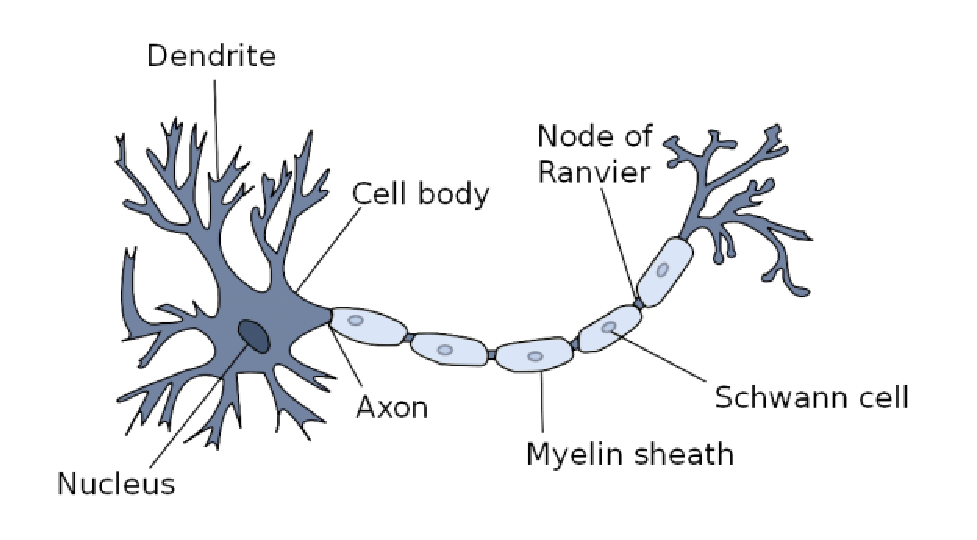
\includegraphics[scale = 0.5]{neuron.eps}
			
			\caption{}
			\label{fig:neuron}
		\end{figure}
		
		\begin{figure}[H]
			\center
			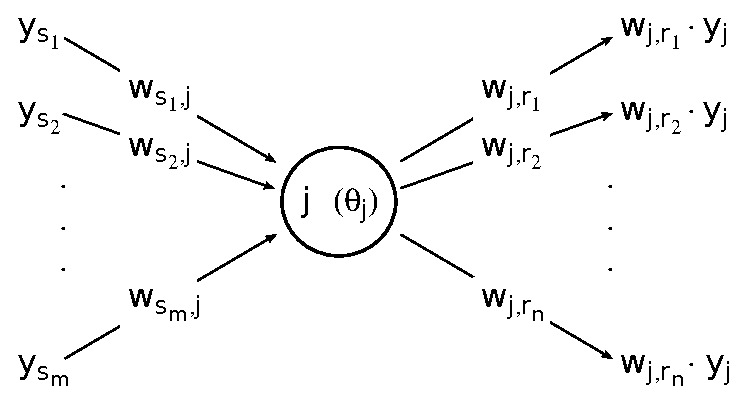
\includegraphics[scale = 0.7]{neural_model_ter.eps}
			
			\caption{}
			\label{fig:neural-model}
		\end{figure}
		
		\begin{figure}[H]
			\center
			\includegraphics[scale = 0.7]{neural_model_bias.eps}
			
			\caption{}
			\label{fig:neural-model-bias}
		\end{figure}
		
		\begin{figure}[H]
			\center
			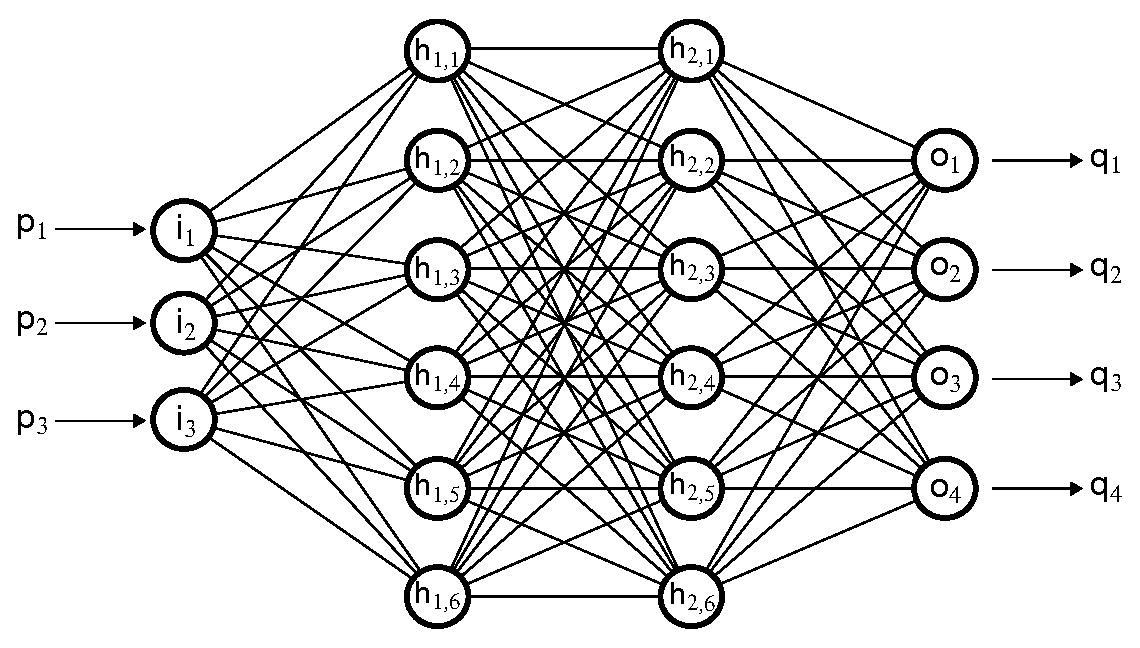
\includegraphics[scale = 0.6]{neural_network_bis.eps}
			
			\caption{}
			\label{fig:neural-network}
		\end{figure}
		
	 
		 
		 
		 

	\chapter{Reduced Basis method for nonlinear elliptic PDEs}
	\label{chapter:Reduced Basis method for nonlinear elliptic PDEs}
	
		In this chapter, we derive a Reduced Basis (RB) approximation for a parametrized Boundary Value problem (BVP) involving a possibly nonlinear elliptic Partial Differential Equation (PDE). As a convenient test case, the nonlinear Poisson equation in one and two spatial dimensions is considered, with the nonlinearity stemming from a solution-dependent viscosity. In the one-dimensional case, the parameters may characterize the viscosity itself, the forcing term, or the boundary conditions. On the contrary, in the two-dimensional framework we are concerned with a parameter-free PDE defined on a domain undergoing geometrical transformations. In the RB context, when dealing with shape variations one needs to introduce a parametric transformation, mapping the whole domain to a parameter-independent reference configuration, e.g. a unit square \cite{MN16}. For this aim, we refer to the boundary displacement-dependent transfinite map (BDD TM) proposed in \cite{JIR14}, building a volumetric parametrization given the boundary parametrization of the domain. 
		
		For the sake of numerical efficiency, the RB procedure is usually carried out within an offline-online framework. The \emph{offline} stage consists in generating the reduced basis out of an ensemble of \emph{snapshots}, i.e. high-fidelity numerical solutions to the BVP for different realizations of the parameters. In this thesis, the well-known Proper Orthogonal Decomposition (POD) technique is used, relying on the Finite Element (FE) method for the computation of the snapshots. Then, given new values for the parameters, in the \emph{online} phase one seeks an approximation to the high-fidelity solution in the reduced space, i.e. the linear space generated by the reduced basis. To retain the well-posedness of the problem, the system yielded by the FE method is projected onto the reduced space, thus enforcing the orthogonality to the reduced basis of the residual for each equation \cite{HRS15,MN16}. Hence, the computational cost associated with the \emph{resolution} of the \emph{reduced} model is \emph{independent} of the size of the original, large-scale model. 
		
		The whole procedure sketched so far is detailed in the following sections. Section \ref{} and \ref{} discuss the Finite Element method applied to the one- and two-dimensional Poisson equation, respectively. The Reduced Basis technique is described in Section \ref{}, while in the final Section \ref{} we present an alternative, Neural Network-based approach for the computation of the reduced solution, which represents the actual novelty of the proposed reduced order modeling algorithm.
		
	\section{Finite Element method for one-dimensional Poisson}
	\label{section:Finite Element method for one-dimensional Poisson}
		
		
	\begin{thebibliography}{50}
	
		\bibitem{Cyb88}
		G. Cybenko. \emph{Continuous valued neural networks with two hidden layers are sufficient}. Technical Report, Department of Computer Science, Tufts University, 1988.
		
		\bibitem{Cyb89}
		G. Cybenko. \emph{Approximation by superpositions of a sigmoidal function}. Mathematics of Control, Signals, and Systems, 2(4):303–314, 1989.
		
		\bibitem{Fah88}
		S. E. Fahlman. \emph{An empirical study of learning speed in back-propagation networks}. Technical Report CMU-CS-88-162, CMU, 1988.
		
		\bibitem{Hag94}
		M. T. Hagan, M. B. Menhaj. \emph{Training feedforward networks with the Marquardt algorithm}. IEEE Transactions on Neural Networks, 5(6):989-993, 1994.
		
		\bibitem{Hag14}
		M. T. Hagan, H. B. Demuth, M. H. Beale, O. De Jes\'us. \emph{Neural Network Design, 2nd Edition}. eBook, 2014.
		
		\bibitem{Hay05}
		S. Haykin. \emph{Neural Networks: A comprehensive foundation}. Prentice Hall, Upper Saddle River, NJ, 2004.
		
		\bibitem{Heb49}
		D. O. Hebb. \emph{The organization of behaviour: A neuropsychological theory}. John Wiley \& Sons, New York, NY, 1949. 
		
		\bibitem{KLM96}
		L. P. Kaelbling, M. L. Littman, A. W. Moore. \emph{Reinforcement Learning: A Survey}. Journal of Artificial Intelligence Reserch, 4:237-285, 1996.
		
		\bibitem{Kri}
		D. Kriesel. \emph{A Brief Introduction to Neural Networks}. \url{http://www.dkriesel.com/en/science/neural_networks}.
		
		\bibitem{Mar63}
		D. W. Marquardt. \emph{An algorithm for least-squares estimation of nonlinear parameters}. Journal of the Society for Industrial and Applied Mathematics, 11(2):431-441, 1963.
				
		\bibitem{MR86}
		J. L. McClelland, D. E. Rumelhart. \emph{Parallel Distributed Processing: Explorations in the Microstructure of Cognition}. MIT Press, Cambridge, UK, 1986.
		
		\bibitem{Nie15}
		M. A. Nielsen. \emph{Neural Networkd and Deep Learning}. Determination Press, 2015.
		
		\bibitem{RB93}
		M. Riedmiller, H. Braun. \emph{A direct adaptive method for faster backpropagation learning: The rprop algorithm}. Neural Networks, IEEE International Conference on, 596-591, 1993.
		
		\bibitem{Ros58}
		F. Rosenblatt. \emph{The perceptron: A probabilistic model for information storage and organization in the brain}. Psychological Review, 65:386-408, 1958.
		
		\bibitem{SD}
		C. Stergiou, D. Siganos. \emph{Neural Networks}. \url{https://www.doc.ic.ac.uk/~nd/surprise_96/journal/vol4/cs11/report.html#Introduction to neural networks}.
		
		\bibitem{WH60}
		B. Widrow, M. E. Hoff. \emph{Adaptive switching circuits}. Proceedings WESCON, 96-104, 1960.
		
	\end{thebibliography}	
	
\end{document}
